\chapter{\label{app:benchmark} Benchmarking}

\minitoc

In order to verify that the simulations performed give reasonable estimates of direct drive experimental performance, the simulation code and settings used were benchmarked by simulating previously performed direct drive experiments. This benchmarking was not intended to be exhaustive, as the results presented in this paper are only meant to be taken as an indication of the performance possible in a new regime, but should serve to demonstrate that simulations performed in this code and with these settings can be used to describe such implosions.

\section{Direct-drive Omega shots}

10 calibration shots performed in a direct-drive configuration on OMEGA for a study of diffusion-dominated mixing were simulated \cite{Zylstra2018a}. The capsules used in these shots consisted of different HT vapour mixtures, surrounded by either pure CH or CH with 2\% D shells (these shells were homogeneous, and did not have a layer structure such as those presented in the paper referenced). Each of the ten shots was simulated using the parameters described in section \ref{Sim Details}, including the 0.8 multiplier to the laser power used to account for CBET. For each of the 10 experimental shots the laser energy absorbed, DT and TT yields were measured, while the bang time and burn width were recorded for 3 of the shots.

\begin{figure}[ht]
\centering
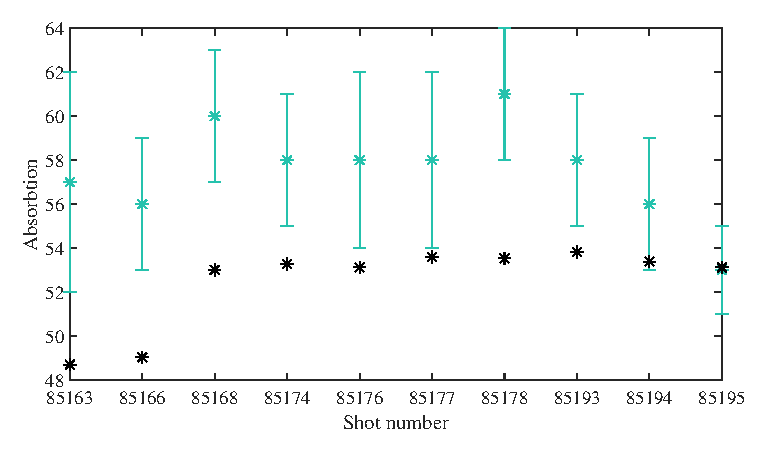
\includegraphics{figures/LowCR/BenchmarkOmegaAbsorbtion.eps}
\caption{Fractional absorption of the laser energy. The orange/grey points are the simulated data, while the blue/black points are the experimental data. The simulated data is obtained by measuring the absorption within the simulation, and multiplying this value by the 0.8 input power multiplier used to account for CBET.}
\label{fig:OmegaAbs}
\end{figure}

\begin{figure}[ht]
\centering
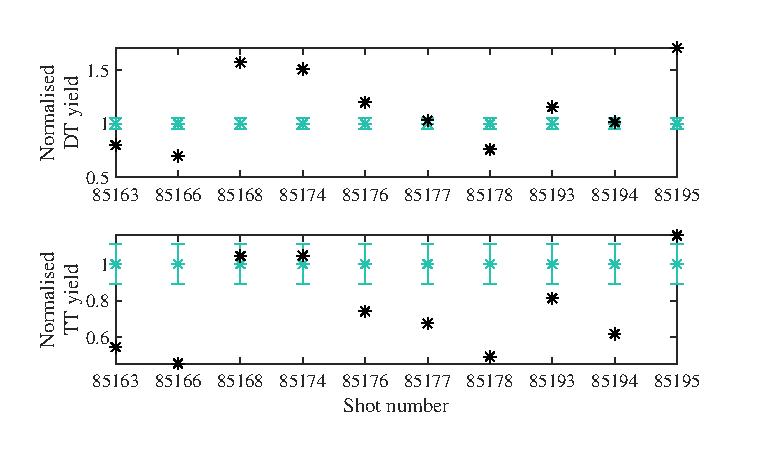
\includegraphics{figures/LowCR/BenchmarkOmegaYield.eps}
\caption{DT and TT yields for the different OMEGA shots, normalised to the experimental data. The orange/grey points are the normalised simulated data, while the blue/black points with a consistent value of 1 are the normalised experimental data, included to show the error bars.}
\label{fig:OmegaYield}
\end{figure}

Figure \ref{fig:OmegaAbs} shows the fractional laser absorption. It is clear that the simulated absorption is typically just outside of the error of the experimental absorbtion, giving a slightly lower value. This could be improved by increasing the value of the CBET multiplier, but given the reasonable agreement between the two (and the fact that high accuracy is not expected or required from this 1D code) it was decided that this constituted an acceptable level of agreement. Figure \ref{fig:OmegaYield} shows the simulated DT and TT yields, normalised to the experimental data, for each of the 10 shots. The normalised DT yield has a mean of 1.14 and varies between approximately 0.7 and 1.7, while the normalised TT yield has a mean of 0.76 and varies between approximately 0.4 and 1.2. Again, given that HYADES is a 1D code, this is a reasonable level of agreement for the purposes of this paper, suggesting that the code and settings used are sufficient to give a reasonable estimate of the obtainable yield. It is notable that while the DT yield is a slight overestimate, the TT yield is a significant underestimate. This could be explained by kinetic effects such as fuel stratification \cite{Bellei2014}, which are not included in hydrodynamic codes and are known to lead to increased TT yields compared to when this effect is not modelled \cite{Casey2012}.

\begin{figure}[ht]
\centering
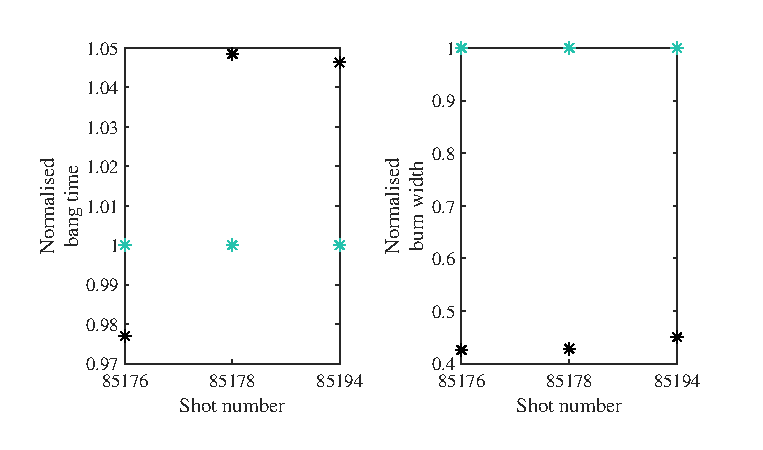
\includegraphics{figures/LowCR/BenchmarkOmegaBT.eps}
\caption{Bang time and burn width for the different OMEGA shots, normalised to the experimental value. The orange/grey points are the normalised simulated data, while the blue/black points with a consistent value of 1 are the normalised experimental data.}
\label{fig:OmegaBT}
\end{figure}


Figure \ref{fig:OmegaBT} shows the normalised bang time and burn width. The bang time displays very good agreement, varying between approximately 0.97 and 1.05. The burn width is significantly underestimated, with all simulated values being around 0.4 to 0.5 times that of the experimental data. The disagreement in burn width is unexplained, but is likely due to a difference between the definition used in simulating it (the FWHM of neutron rate) and in the experiment (which was unknown to the authors of this work). Given the success of the code in simulating the more important parameters (particularly the DT yield and bang time), it was decided that these results were satisfactory to show that Hyades could be used with these settings to simulate direct-drive implosions.

\section{Polar direct-drive NIF shot}

The polar direct drive NIF shot N190227 \cite{NIFshot} was also simulated. This capsule had a 3943~\si[per-mode=symbol]{\micro\meter} outer diameter and a 25~\si[per-mode=symbol]{\micro\meter} CH ablator, and was filled with 6000 torr DT (64\% D, 36\%T). The laser ramped linearly from 0 to 400 TW over 1.5ns, remained at this power for 2 ns, and then decreased to 0 TW over 0.5 ns. The simulation parameters were unchanged from those used for the OMEGA shots. A range of input power multipliers were used, as the absorption was expected to be lower due to the PDD configuration. This shot produced a DT yield of \num{1.11e16} neutrons (no error was given for this value), a bang time of 4.51 $\pm$ 0.03 ns, and a burn width of 468 $\pm$ 50 ps. 

\begin{figure}[ht]
\centering
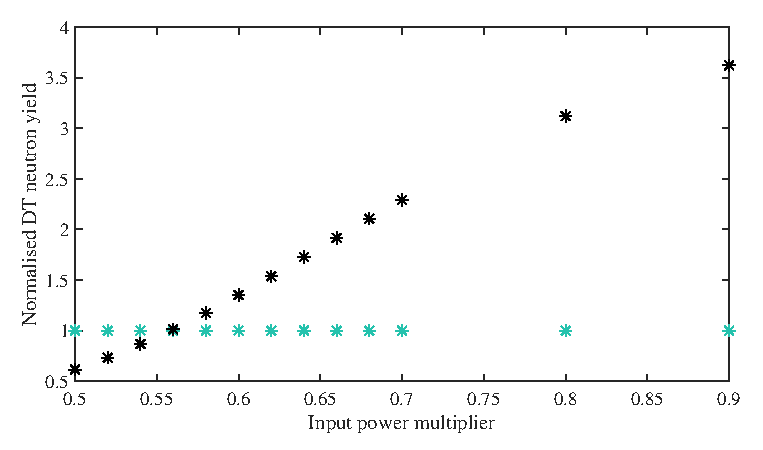
\includegraphics{figures/LowCR/BenchmarkNifYield.eps}
\caption{DT yield for NIF shot N190227 simulated using a range of input power multipliers, normalised to the experimental value of \num{1.11e16}. The orange/grey points are the normalised simulated data, while the blue/black points with a consistent value of 1 are the normalised experimental data.}
\label{fig:NIFYield}
\end{figure}

\begin{figure}[ht]
\centering
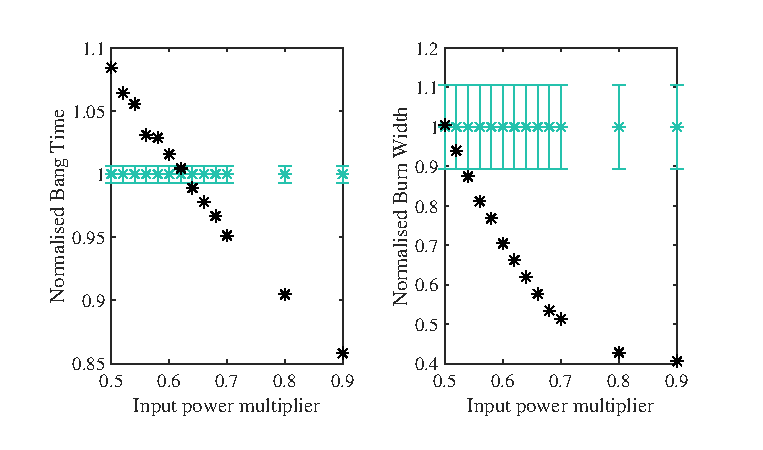
\includegraphics{figures/LowCR/BenchmarkNifBangTime.eps}
\caption{Bang time and burn width for NIF shot N190227 simulated using a range of input power multipliers, normalised to the experimental values of 4.51 $\pm$ 0.03 ns and 468 $\pm$ 50 ps respectively. The orange/grey points are the normalised simulated data, while the blue/black points with a consistent value of 1 are the normalised experimental data.}
\label{fig:NIFBT}
\end{figure}

The normalised DT yield for the different input power multipliers can be seen in figure \ref{fig:NIFYield}. Reasonable agreement is seen for lower value input multipliers, with the best agreement observed for multipliers between 0.54 and 0.58. The multiplier of 0.8 used for the OMEGA work gives a DT yield for the NIF shot approximately three times higher than that measured experimentally. The normalised bang time and burn width can be seen in figure \ref{fig:NIFBT}. The normalised bang time shows good agreement (between 1.05 and 0.95) for input multipliers ranging from 0.56 to 0.7, although it is closest for around 0.62. The burn width is within the error for an input multiplier of 0.5 to 0.52, and is approximately 0.7 times that of the experimental value for a multiplier of 0.6. These three sets of results together suggest that good agreement can be observed for input multipliers of around 0.55 to 0.6, which is significantly lower than the 0.8 used in the OMEGA simulations.

The requirement for a lower multiplier can most likely be explained by the PDD configuration. As discussed in section \ref{Results}, PDD is particularly susceptible to cross beam energy transfer, which would result in less of the laser energy being absorbed. In addition, as the capsule is compressed, the lasers pointing at the equator in a PDD configuration will no longer be incident on the target, resulting in a fraction of the laser energy not being absorbed. This effect will be most significant at later times where the capsule radius is smallest, which is also when the maximum power is applied. This likely explains the need for a lower multiplier, and so it is worth bearing in mind that the 0.8 multiplier used in the simulation campaign is applicable for a symmetric direct drive configuration, but reduced performance should be expected if a PDD configuration is used instead (or that an input power around 30\% higher would be needed to achieve equivalent performance, along with the associated increase in energy).

These results appear sufficient to suggest that Hyades can be used to gain a reasonable indication of the performance for direct-drive implosions, as it is used for in this paper. This benchmarking is not exhaustive, and could be expanded by looking at more complicated capsule designs. In particular, simulations involving wetted foam capsules would be useful, as this would give some indication of how significant the presence of the CH foam is, and increased confidence in the results. As this paper considers only 1D simulations (and uses them only for an initial exploration of a new regime), it was decided that the benchmarking seen here was satisfactory to demonstrate that Hyades can be used for this application.
